\subsubsection{NASA-TLX}
\label{subsubsec:results_nasa_tlx_1}

The NASA-TLX provides two information that are relevant to the workload analysis. The first one is the score attributed to the ‘mental demand’ dimension. The second one is the average obtained from the scores of the six dimensions of NASA-TLX. The two analyses are presented in the next subsections.

\paragraph{Analysis of the mental demand scale}\mbox{}\\

Table \ref{tab:md_table_blind} presents the ‘mental demand’ score attributed by each blind participant to each guidance method. The ‘base’ method refers to the guidance method that the person uses in his/her daily life (e.g., white cane). 


\begin{table}[!htb]
\centering
\caption{Score of NASA-TLX mental demand for the blind participants.}
\label{tab:md_table_blind}
\begin{tabular}{llrrrrr}
\toprule
     &        & Base & Audio & \begin{tabular}[c]{@{}l@{}}Haptic\\ Belt\end{tabular} & \begin{tabular}[c]{@{}l@{}}Virtual\\ Cane\end{tabular} & Mixture \\
Participant & Round &      &       &                                                       &                                                        &         \\
\midrule
001C & First &    3 &     1 &                                                    14 &                                                      3 &       6 \\
     & Return &    1 &     1 &                                                    10 &                                                      2 &       6 \\
002C & First &    5 &     1 &                                                     1 &                                                     10 &      12 \\
     & Return &    1 &     1 &                                                     1 &                                                     10 &       3 \\
003C & First &    5 &     5 &                                                     5 &                                                      8 &       1 \\
     & Return &    3 &     1 &                                                     1 &                                                      2 &       1 \\
004C & First &    9 &    10 &                                                    15 &                                                     10 &      10 \\
     & Return &    7 &    10 &                                                    14 &                                                      8 &      10 \\
\bottomrule
\end{tabular}
\end{table}



The mean value obtained for each guidance method is illustrated in Figure \ref{fig:barplot_md_avg_5_scene_blind}. It shows a systematic reduction on the perceived mental workload between the rounds for all methods, confirming that the participants get familiar with the devices after the first use. It also shows that although the haptic belt obtained the largest mean, it also had the largest variation, showing that the effort required from the user may vary significantly.

\begin{figure}[!htb]
    \centering
    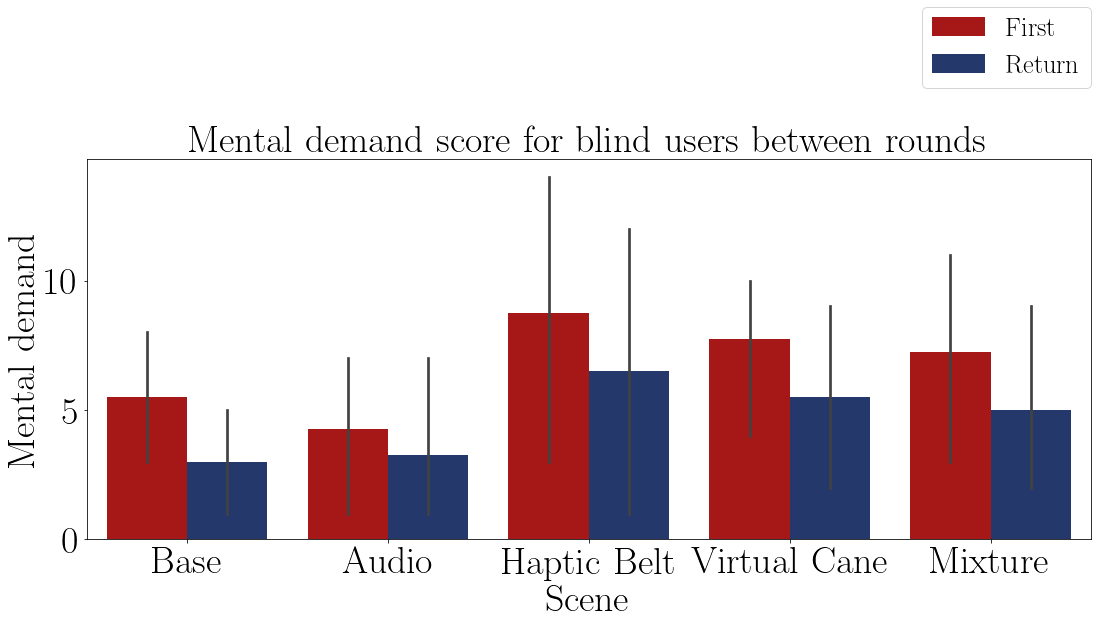
\includegraphics[width = 0.8\linewidth]{Resultados/Nasa/Figuras/png/barplot_md_avg_5_scene_blind.png}
    \caption{Barplot of the average mental demand of the blind participants on each method.}
    \label{fig:barplot_md_avg_5_scene_blind}
\end{figure}

Figure \ref{fig:boxplot_md_blind_scene}  presents a box plot of the mental demand score grouped by method. This Figure shows that there may be two different groups: one associated with lower demand, composed of ‘base’ and ‘audio’, and another with higher demand, composed of ‘haptic belt’, ‘virtual cane’ and ‘mixture’. It indicates that maybe a guidance method that uses vibration as input is not intuitive. Following, Figure \ref{fig:boxplot_md_blind_rounds} presents a box plot of the mental demand grouped by the rounds, confirming the general tendency to reduce the required ‘mental demand’. 

\begin{figure}[!htb]
    \centering
    \begin{minipage}{0.45\textwidth}
        \centering
        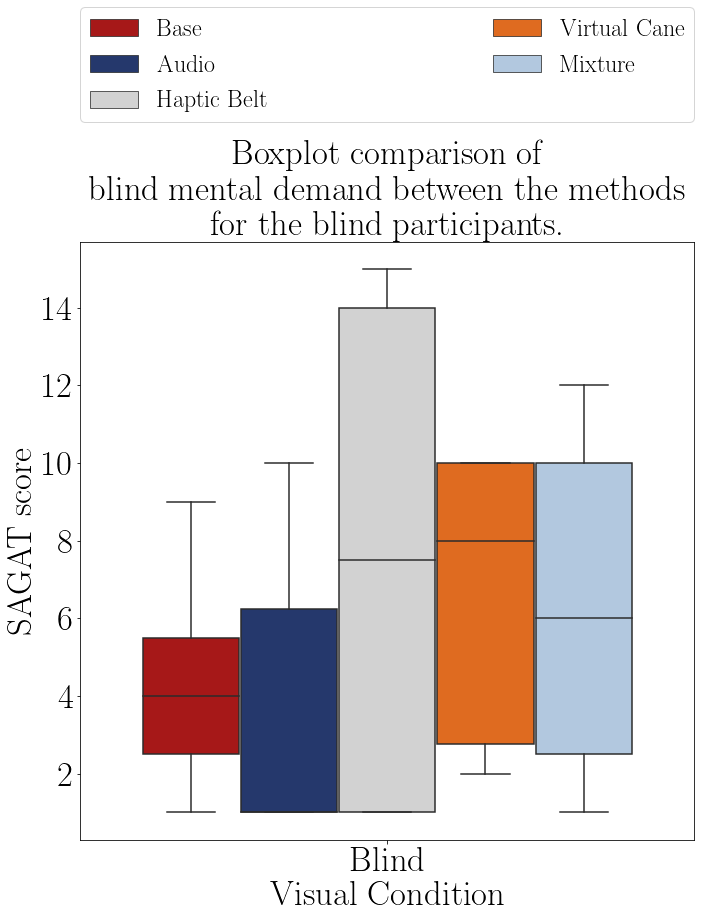
\includegraphics[width = 0.8\linewidth]{Resultados/Nasa/Figuras/png/boxplot_md_blind_scene.png}
        \caption{Boxplot of the mental demand of the blind participants grouped by method.}
        \label{fig:boxplot_md_blind_scene}
    \end{minipage}
    \begin{minipage}{0.45\textwidth}
        \centering
        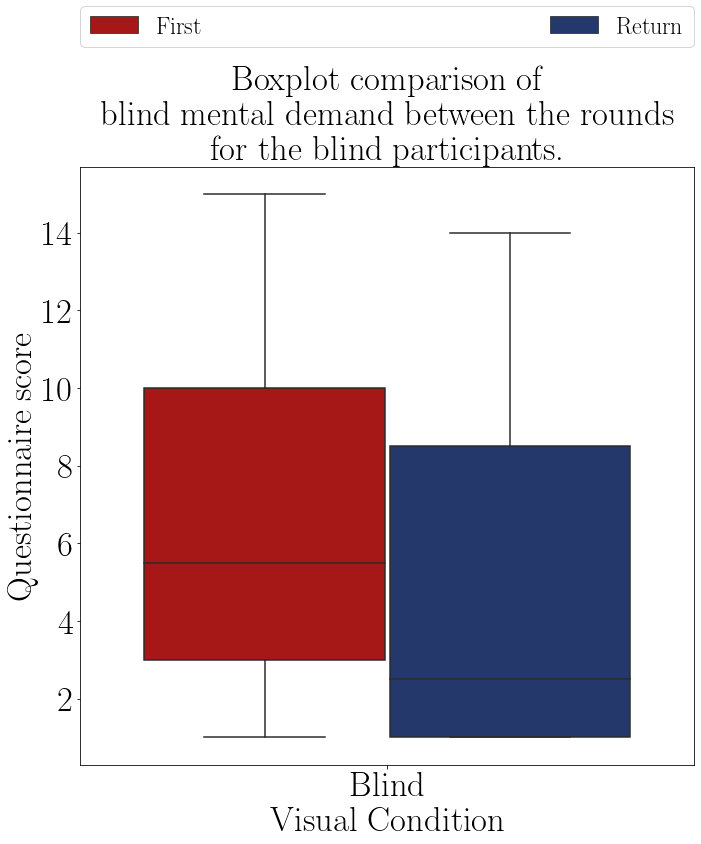
\includegraphics[width = 0.8\linewidth]{Resultados/Nasa/Figuras/png/boxplot_md_blind_rounds.png}
        \caption{Boxplot of the mental demand of the blind participants grouped by round.}
        \label{fig:boxplot_md_blind_rounds}
    \end{minipage}
\end{figure}

In order to support the statistical analysis, Figures \ref{fig:qqplot_md_avg_two_way_blind} and \ref{fig:residplot_md_avg_two_way_blind} presents the QQ-plot and the residual plot of the ‘mental demand’ data, confirming that the data follow a normal distribution and the residues are homogenous.

Following, Figures \ref{fig:qqplot_md_avg_two_way_blind} and \ref{fig:residplot_md_avg_two_way_blind} shows the distribution and variance of the Table \ref{tab:md_table_blind}. These Figures shows that the data are normally distributed and that the methods have a similar variance. The Table \ref{tab:blocanova_md_avg_two_way_blind} shows the Anova test p-values of the mental demand of the ‘blind” sample between the guidance methods. The method’s and the round’s p-values indicates that there is no influence from them in the mental demand. The interaction between the methods and the round also does not influences the mental demand.

\begin{figure}[!htb]
    \centering
    \begin{minipage}{0.45\textwidth}
        \centering
        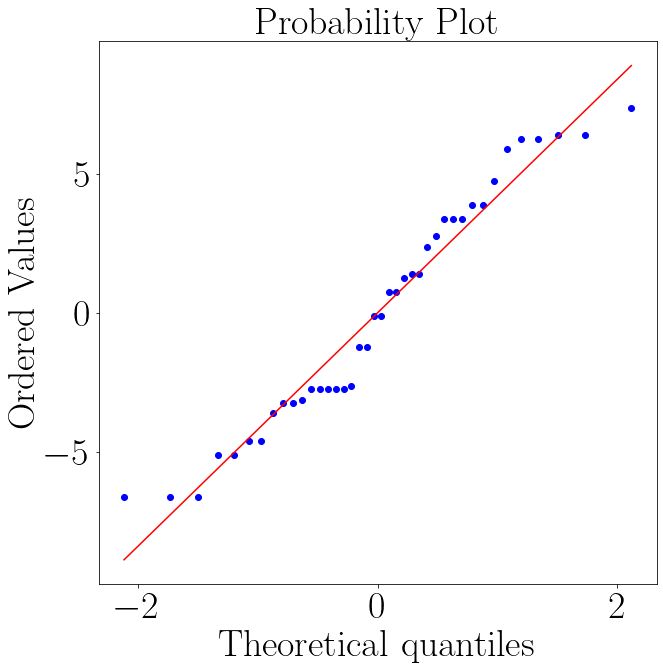
\includegraphics[width = 0.8\linewidth]{Resultados/Nasa/Figuras/png/qqplot_md_avg_two_way_blind.png}
        \caption{QQ plot of the mental demand of the blind participants on each method.}
        \label{fig:qqplot_md_avg_two_way_blind}
    \end{minipage}
    \begin{minipage}{0.45\textwidth}
        \centering
        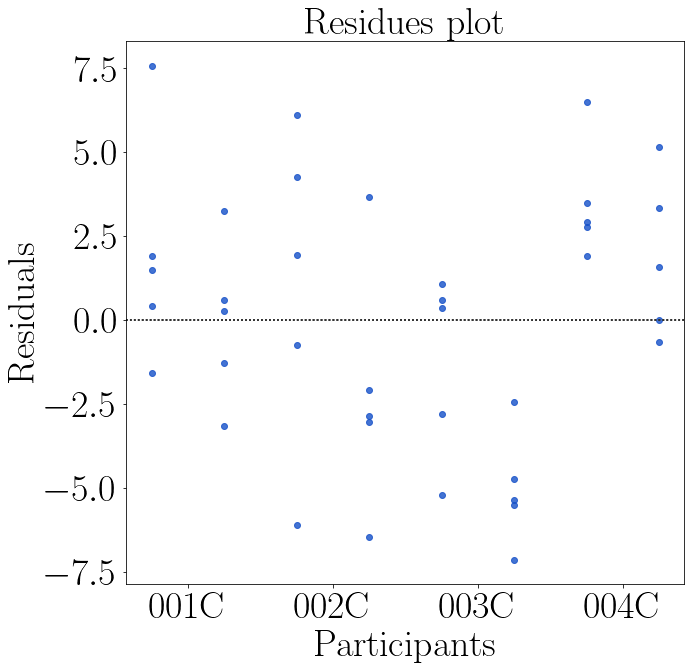
\includegraphics[width = 0.8\linewidth]{Resultados/Nasa/Figuras/png/residplot_md_avg_two_way_blind.png}
        \caption{Residual plot of the mental demand score the blind participants on each method.}
        \label{fig:residplot_md_avg_two_way_blind}
    \end{minipage}
\end{figure}

Following, the statistical model of Equation 5.1 is used for the analysis of variance (ANOVA): 

\begin{equation}
    \label{eq:statistical_model}
    y_{ijk} = \mu + \tau_i + \beta_j +\omega_k + (\tau\beta_{ij}) + e
\end{equation}

where:

\begin{itemize}
    \item $y_{ij}$ - output variable for method $i$, round $j$ and participant $k$;
    \item $\mu$ - mean of all the observations;
    \item $\tau_i$ - variance from method $i$;
    \item $\beta_j$ - variance from round $j$;
    \item $\omega_k$ - variance from participant k, which treated as a block;
    \item $e_{ij}$ - Is observation's residue.
\end{itemize}


\begin{table}[!htb]
\centering
\caption{Anova p-value for the mental demand average on each method for blinded users.}
\label{tab:blocanova_md_avg_two_way_blind}
\begin{tabular}{lrrrrl}
\toprule
               Source &  Squared sum &  DOF & Squared average &     F & \begin{tabular}[c]{@{}l@{}}P-Value \\ $(F_{0} > F)$\end{tabular} \\
\midrule
Participants (Blocks) &      298.475 &    3 &          99.492 & 8.133 &                                                                  \\
         \    Methods &       85.150 &    4 &          21.288 & 1.740 &                                                            0.170 \\
          \    Rounds &       42.025 &    1 &          42.025 & 3.436 &                                                            0.075 \\
     \    Interaction &        2.850 &    4 &           0.712 & 0.058 &                                                            0.993 \\
   Experimental Error &      330.275 &   27 &          12.232 &       &                                                                  \\
                Total &      758.775 &   39 &                 &       &                                                                  \\
\bottomrule
\end{tabular}
\end{table}



%The Table \ref{tab:lsdtwoway_md_avg_two_way} presents the conclusion of a pairwise Fisher LSD test of the blind mental demand between all the guidance methods. The results show that only the "Audio" has a similar mental demand as the "Base" method.

%\input{Resultados/Nasa/Tabelas/lsdtwoway_md_avg_two_way.tex}

The Table \ref{tab:md_var_average_group_blind} shows the average of the mental demand variation between the rounds. This table shows that the mental demand variation from the “Audio” has the lower variation, and the rest are similar variations.


\begin{table}[!htb]
\centering
\caption{Mental demand variation grouped by participant and visual condition}
\label{tab:md_var_average_group_blind}
\begin{tabular}{lrrrrrr}
\toprule
{} &  Base & Audio & \begin{tabular}[c]{@{}l@{}}Haptic\\ Belt\end{tabular} & \begin{tabular}[c]{@{}l@{}}Virtual\\ Cane\end{tabular} & Mixture \\
Visual Condition &       &       &                                                       &                                                        &         \\
\midrule
Blind            &  -2.5 &  -1.0 &                                                  -2.2 &                                                   -2.2 &    -2.2 \\
\bottomrule
\end{tabular}
\end{table}



The Figures \ref{fig:qqplot_md_var_blind} and \ref{fig:residplot_md_var_blind} shows the distribution and variance of the mental demand variation of the Table \ref{tab:md_table_blind}. These Figures shows that the data are normally distributed and that the methods have a similar variance.
The Table \ref{tab:blocanova_md_var_blind} shows the Anova test p-value of the mental demand of the "blind" sample between the guidance methods. The p-value indicates that there is no influence of the methods in the variation of mental demand between the rounds. 


\begin{table}[!htb]
\centering
\caption{Anova p-value for the mental demand variation on each method for blinded users.}
\label{tab:blocanova_md_var_blind}
\begin{tabular}{lrrrrr}
\toprule
               Source &  Squared sum &  DOF & Squared average &     F & \begin{tabular}[c]{@{}l@{}}P-Value \\ $(F_{0} > F)$\end{tabular} \\
\midrule
Participants (blocks) &       15.750 &    3 &           1.425 & 0.674 &                                                                  \\
               Method &        5.700 &    4 &           5.250 & 0.183 &                                                            0.943 \\
   Experimental error &       93.500 &   12 &           7.792 &       &                                                                  \\
                Total &      114.950 &   19 &                 &       &                                                                  \\
\bottomrule
\end{tabular}
\end{table}



\begin{figure}[!htb]
    \centering
    \begin{minipage}{0.45\textwidth}
        \centering
        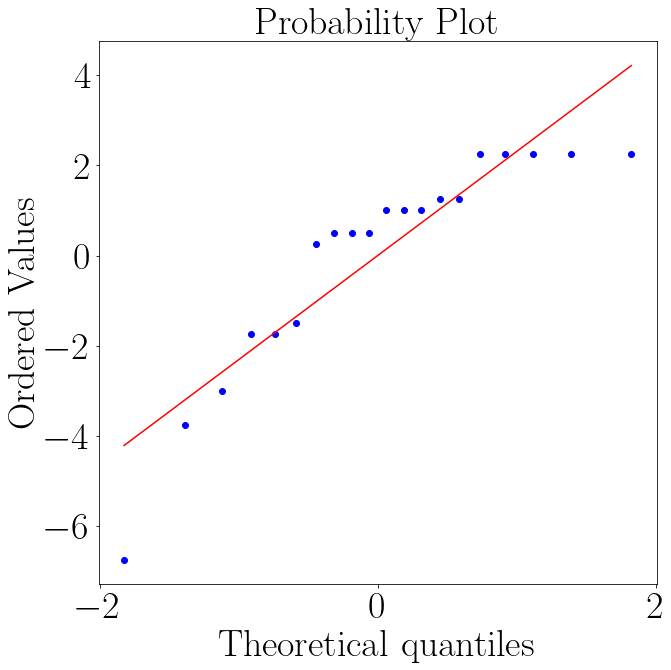
\includegraphics[width = 0.8\linewidth]{Resultados/Nasa/Figuras/png/qqplot_md_var_blind.png}
        \caption{Residual plot of the mental demand variation of the blind participants on each method.}
        \label{fig:qqplot_md_var_blind}
    \end{minipage}
    \begin{minipage}{0.45\textwidth}
        \centering
        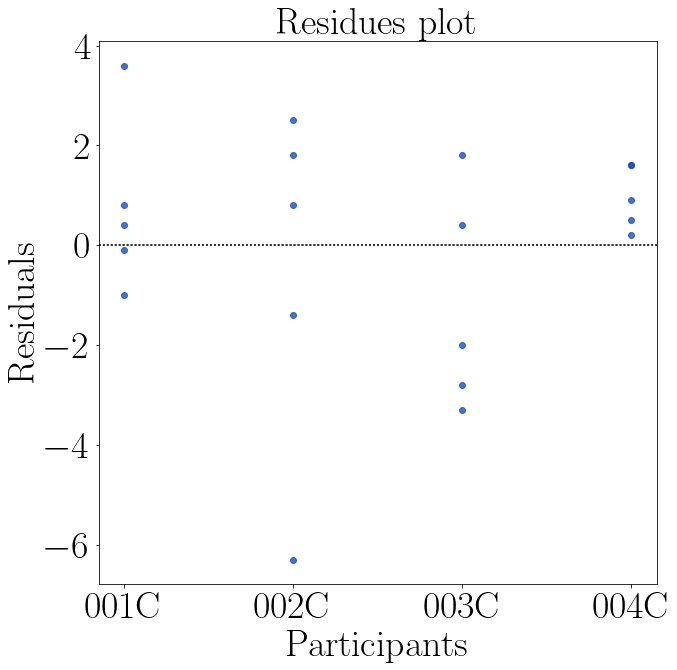
\includegraphics[width = 0.8\linewidth]{Resultados/Nasa/Figuras/png/residplot_md_var_blind.png}
        \caption{Residual plot of the mental demand variation of the sighted participants on each method.}
        \label{fig:residplot_md_var_blind}
    \end{minipage}
\end{figure}

%The Table \ref{tab:lsdbloc_mental_demand_var} presents the conclusion of a pairwise Fisher LSD test of the blind mental demand between all the guidance methods. The results show that all methods have similar variations.

%
\begin{table}[!htb]
\centering
\caption{Cross validation p-value for the mental demand variation on each method for blinded users.}
\label{tab:lsdbloc_mental_demand_var}
\begin{tabular}{rclr}
\toprule
      \multicolumn{3}{c}{Method} &                                       Analysis \\
\midrule
              Base & $X$ & Audio &           $H_1 : \mu_{Base} \ne \mu_{Audio}**$ \\
        Base & $X$ & Haptic Belt &         $H_0 : \mu_{Base} = \mu_{Haptic Belt}$ \\
       Base & $X$ & Virtual Cane &    $H_1 : \mu_{Base} \ne \mu_{Virtual Cane}**$ \\
            Base & $X$ & Mixture &         $H_1 : \mu_{Base} \ne \mu_{Mixture}**$ \\
       Audio & $X$ & Haptic Belt &    $H_1 : \mu_{Audio} \ne \mu_{Haptic Belt}**$ \\
      Audio & $X$ & Virtual Cane &       $H_0 : \mu_{Audio} = \mu_{Virtual Cane}$ \\
           Audio & $X$ & Mixture &            $H_0 : \mu_{Audio} = \mu_{Mixture}$ \\
Haptic Belt & $X$ & Virtual Cane & $H_0 : \mu_{Haptic Belt} = \mu_{Virtual Cane}$ \\
     Haptic Belt & $X$ & Mixture &  $H_1 : \mu_{Haptic Belt} \ne \mu_{Mixture}**$ \\
    Virtual Cane & $X$ & Mixture &     $H_0 : \mu_{Virtual Cane} = \mu_{Mixture}$ \\
\bottomrule
\end{tabular}
\end{table}



To close up, according to the ANOVA test at Table \ref{tab:blocanova_md_avg_two_way_blind} there is no influence in the tested methods in the participants mental demand, but at the Figure \ref{fig:boxplot_md_blind_scene} it is posible to notice that there is at least two different groups of mental demand reactions, one formed by the "Base" and the "Audio" methods and another formed by the rest of the methods. The first group has lower mental demand than the last. That could mean that the presence of a haptic device increases the mental demand of the navigation activity for the BVI users. This was not reflected in the ANOVA results because of the small sample size.

\FloatBarrier

%%%%%%%%%%%%%%%%%%%%%%%%%%%%%%%%%%%%%%%%%%%%%%%%%%%%%%%%%%%%%%%%%%%%%%%%%%%
%%%%%%%%%%%%%%%%%%%%%%%%%%%%%%%%%%%%%%%%%%%%%%%%%%%%%%%%%%%%%%%%%%%%%%%%%%%
%%%%%%%%%%%%%%%%%%%%%%%%%%%%%%%%%%%%%%%%%%%%%%%%%%%%%%%%%%%%%%%%%%%%%%%%%%%
%%%%%%%%%%%%%%%%%%%%%%%%%%%%%%%%%%%%%%%%%%%%%%%%%%%%%%%%%%%%%%%%%%%%%%%%%%%


\paragraph{Analysis of the NASA-TLX score}\mbox{}\\

The Table \ref{tab:nasa_table_blind} presents the NASA-TLX score averages by each blinded participant on each scene and they are plotted in the Figures \ref{fig:barplot_nasa_avg_5_scene_blind}. The Figure \ref{fig:barplot_nasa_avg_5_scene_blind} shows a similar behaviour of the mental demand barplot at Figure \ref{fig:barplot_md_avg_5_scene_blind}, all NASA-TLX score decreased from the "First" to the "Return" round. This a kind of learning between the rounds.


\begin{table}[!htb]
\centering
\caption{NASA-TLX score felled by the blinded participants.}
\label{tab:nasa_table_blind}
\begin{tabular}{llrrrrr}
\toprule
     &        &  Base &  Audio & \begin{tabular}[c]{@{}l@{}}Haptic\\ Belt\end{tabular} & \begin{tabular}[c]{@{}l@{}}Virtual\\ Cane\end{tabular} & Mixture \\
Participant & Round &       &        &                                                       &                                                        &         \\
\midrule
001C & First & 4.833 &  4.000 &                                                 8.833 &                                                  5.167 &   6.333 \\
     & Return & 4.167 &  4.000 &                                                 6.667 &                                                  4.500 &   6.167 \\
002C & First & 6.333 &  4.833 &                                                 4.833 &                                                  9.000 &   7.000 \\
     & Return & 4.500 &  4.833 &                                                 4.833 &                                                  7.000 &   5.167 \\
003C & First & 4.000 &  4.000 &                                                 5.333 &                                                  6.667 &   3.500 \\
     & Return & 4.000 &  3.833 &                                                 3.667 &                                                  3.500 &   3.500 \\
004C & First & 9.833 & 10.000 &                                                12.667 &                                                  9.667 &  11.000 \\
     & Return & 8.667 &  9.167 &                                                11.667 &                                                  9.333 &  10.833 \\
\bottomrule
\end{tabular}
\end{table}



\begin{figure}[!htb]
    \centering
    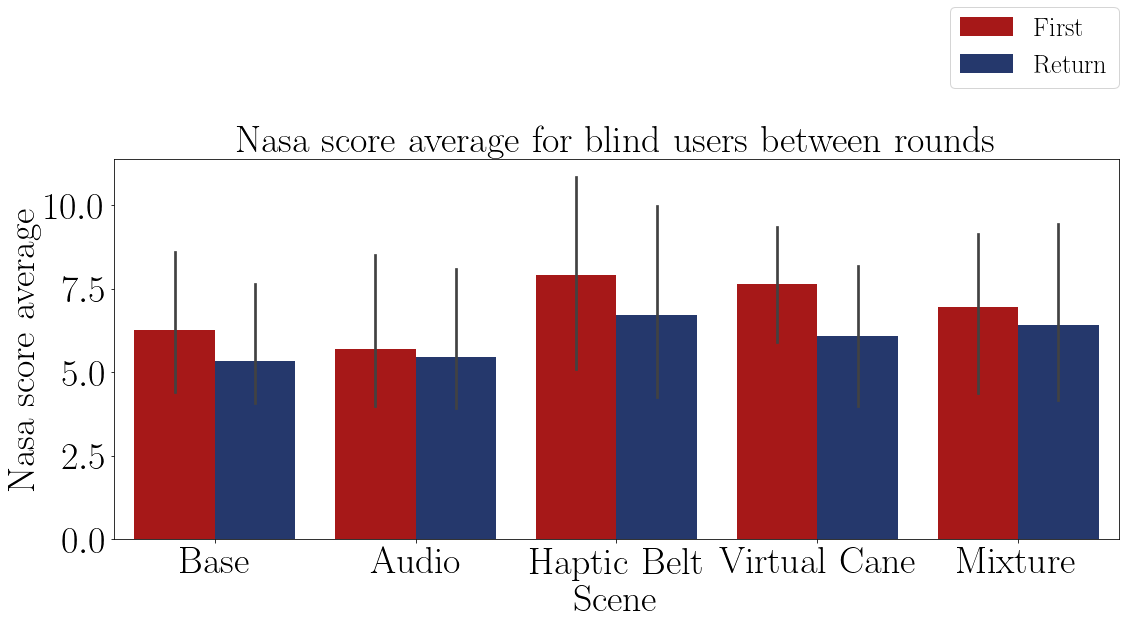
\includegraphics[width = 0.8\linewidth]{Resultados/Nasa/Figuras/png/barplot_nasa_avg_5_scene_blind.png}
    \caption{Barplot of the average NASA-TLX score of the blind participants on each method.}
    \label{fig:barplot_nasa_avg_5_scene_blind}
\end{figure}

The Figure \ref{fig:boxplot_nasa_blind_scene} presents a box plot with the NASA-TLX score grouped by method. This Figure shows it is possible to split the methods in two different groups, one with lower demand formed by the "Base" and the "Audio" method, and another with the higher demand, similar as it was with the mental demand in the \ref{fig:boxplot_md_blind_scene}. It appears that the presence of the an haptic device elevated the NASA-TLX score. The Figure \ref{fig:boxplot_nasa_blind_rounds} presents a box plot with the NASA-TLX score grouped by the rounds. This figure shows that both rounds have similar variations.

\begin{figure}[!htb]
    \centering
    \begin{minipage}{0.45\textwidth}
        \centering
        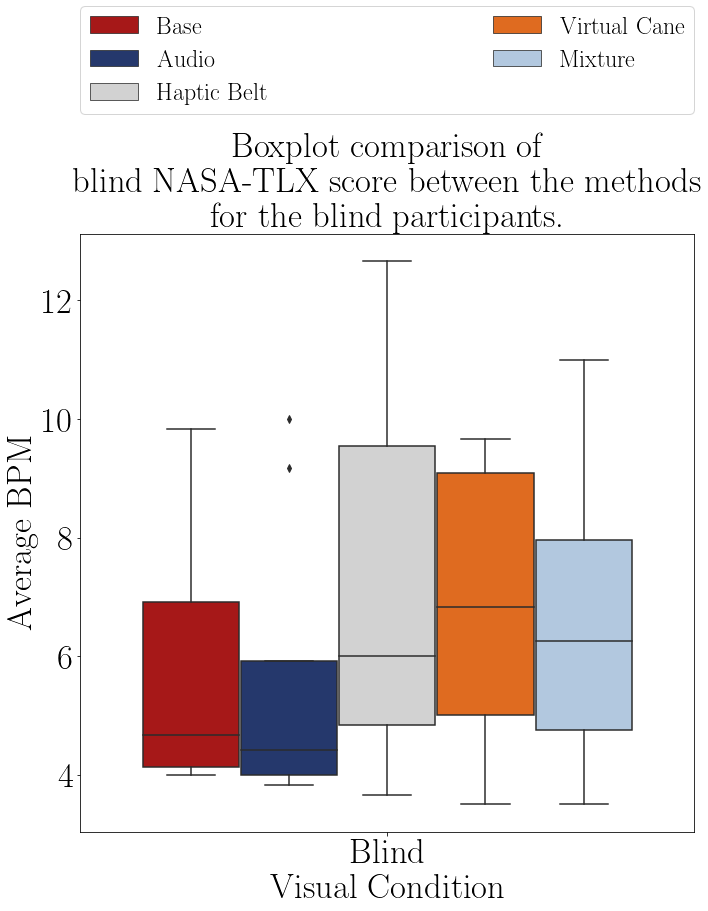
\includegraphics[width = 0.8\linewidth]{Resultados/Nasa/Figuras/png/boxplot_nasa_blind_scene.png}
        \caption{QQ plot of the NASA-TLX score of the blind participants on each method.}
        \label{fig:boxplot_nasa_blind_scene}
    \end{minipage}
    \begin{minipage}{0.45\textwidth}
        \centering
        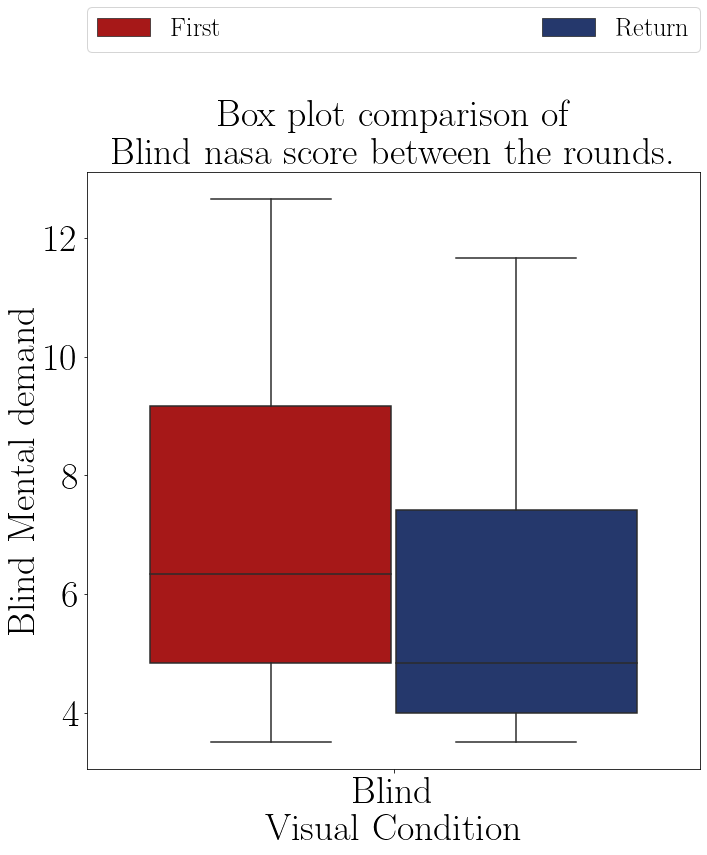
\includegraphics[width = 0.8\linewidth]{Resultados/Nasa/Figuras/png/boxplot_nasa_blind_rounds.png}
        \caption{Residual plot of the NASA-TLX score the blind participants on each method.}
        \label{fig:boxplot_nasa_blind_rounds}
    \end{minipage}
\end{figure}

The Table \ref{tab:nasa_average_group_blind} shows the average NASA-TLX score in the “blind” sample and is possible to notice how the average score by the “blind” sample was lower during the “Audio” and the “Base” methods.


\begin{table}[!htb]
\centering
\caption{Average NASA-TLX score of the blind participants}
\label{tab:nasa_average_group_blind}
\begin{tabular}{lrrrrrr}
\toprule
{} &  Base & Audio & \begin{tabular}[c]{@{}l@{}}Haptic\\ Belt\end{tabular} & \begin{tabular}[c]{@{}l@{}}Virtual\\ Cane\end{tabular} &  Mixture \\
Visual Condition &       &       &                                                       &                                                        &          \\
\midrule
Blind            &  5.79 &  5.58 &                                                  7.31 &                                                   6.85 &    6.688 \\
\bottomrule
\end{tabular}
\end{table}



The Figures \ref{fig:qqplot_nasa_avg_two_way} and \ref{fig:residplot_nasa_avg_two_way} shows the distribution and variance of the Table \ref{tab:nasa_table_blind}. These Figures shows that the data are normally distributed and that the methods have a similar variance.
The Table \ref{tab:blocanova_nasa_avg_two_way} shows the Anova test p-value of the NASA-TLX score of the "blind" sample between the guidance methods. The p-values indicates that some methods have influence on the NASA-TLX score and that the rounds also influences the score. On the other way, their interaction, has no influence on the score.


\begin{table}[!htb]
\centering
\caption{Cross validation p-value for the NASA-TLX score on each method for blinded users.}
\label{tab:blocanova_nasa_avg_two_way}
\begin{tabular}{rclr}
\toprule
      \multicolumn{3}{c}{Method} &                                           Analysis \\
\midrule
              Base & $X$ & Audio &                   $H_0 : \mu_{Base} = \mu_{Audio}$ \\
        Base & $X$ & Haptic Belt &         $H_1 : \mu_{Base} \ne \mu_{Haptic Belt}**$ \\
       Base & $X$ & Virtual Cane &        $H_1 : \mu_{Base} \ne \mu_{Virtual Cane}**$ \\
            Base & $X$ & Mixture &             $H_1 : \mu_{Base} \ne \mu_{Mixture}**$ \\
       Audio & $X$ & Haptic Belt &        $H_1 : \mu_{Audio} \ne \mu_{Haptic Belt}**$ \\
      Audio & $X$ & Virtual Cane &       $H_1 : \mu_{Audio} \ne \mu_{Virtual Cane}**$ \\
           Audio & $X$ & Mixture &            $H_1 : \mu_{Audio} \ne \mu_{Mixture}**$ \\
Haptic Belt & $X$ & Virtual Cane & $H_1 : \mu_{Haptic Belt} \ne \mu_{Virtual Cane}**$ \\
     Haptic Belt & $X$ & Mixture &      $H_1 : \mu_{Haptic Belt} \ne \mu_{Mixture}**$ \\
    Virtual Cane & $X$ & Mixture &         $H_0 : \mu_{Virtual Cane} = \mu_{Mixture}$ \\
\bottomrule
\end{tabular}
\end{table}



\begin{figure}[!htb]
    \centering
    \begin{minipage}{0.45\textwidth}
        \centering
        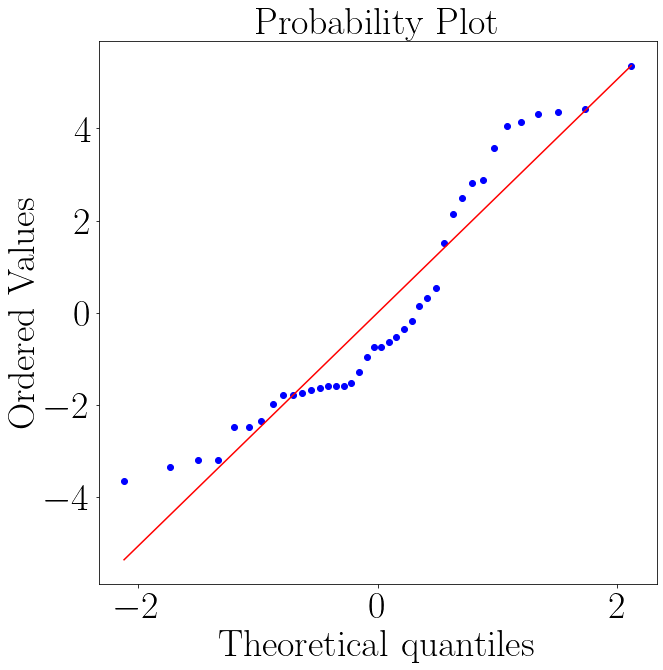
\includegraphics[width = 0.8\linewidth]{Resultados/Nasa/Figuras/png/qqplot_nasa_avg_two_way.png}
        \caption{QQ plot of the NASA-TLX score variation of the blind participants on each method.}
        \label{fig:qqplot_nasa_avg_two_way}
    \end{minipage}
    \begin{minipage}{0.45\textwidth}
        \centering
        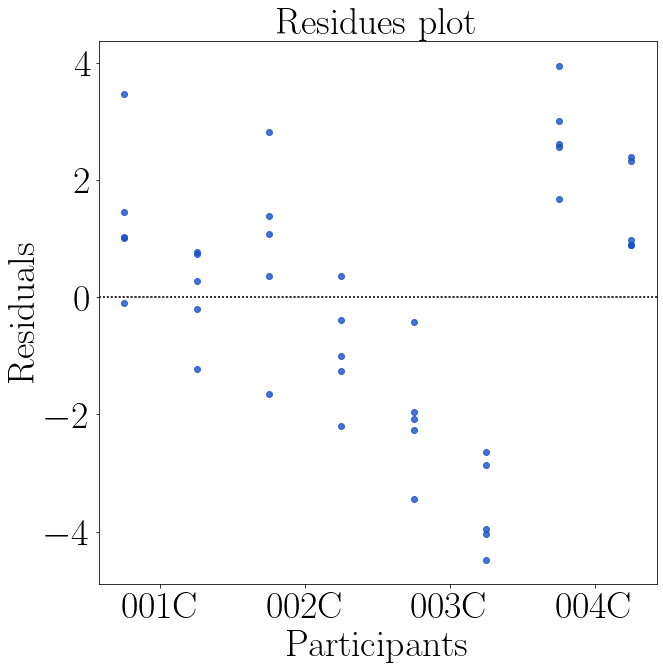
\includegraphics[width = 0.8\linewidth]{Resultados/Nasa/Figuras/png/residplot_nasa_avg_two_way.png}
        \caption{Residual plot of the NASA-TLX score variation the blind participants on each method.}
        \label{fig:residplot_nasa_avg_two_way}
    \end{minipage}
\end{figure}



The Table \ref{tab:lsd_nasa_avg_two_way} presents the conclusion of a pairwise Fisher LSD test of the blind NASA-TLX score between all the guidance methods. The results show that only the "Audio" has a similar NASA-TLX score as the "Base" method, as it was also posible to notice at Figure \ref{fig:boxplot_nasa_blind_scene}.


\begin{table}[!htb]
\centering
\caption{Cross validation p-value for the NASA-TLX score on each method for blinded users.}
\label{tab:lsd_nasa_avg_two_way}
\begin{tabular}{rclr}
\toprule
      \multicolumn{3}{c}{Method} &                                           Analysis \\
\midrule
              Base & $X$ & Audio &                   $H_0 : \mu_{Base} = \mu_{Audio}$ \\
        Base & $X$ & Haptic Belt &         $H_1 : \mu_{Base} \ne \mu_{Haptic Belt}**$ \\
       Base & $X$ & Virtual Cane &        $H_1 : \mu_{Base} \ne \mu_{Virtual Cane}**$ \\
            Base & $X$ & Mixture &             $H_1 : \mu_{Base} \ne \mu_{Mixture}**$ \\
       Audio & $X$ & Haptic Belt &        $H_1 : \mu_{Audio} \ne \mu_{Haptic Belt}**$ \\
      Audio & $X$ & Virtual Cane &       $H_1 : \mu_{Audio} \ne \mu_{Virtual Cane}**$ \\
           Audio & $X$ & Mixture &            $H_1 : \mu_{Audio} \ne \mu_{Mixture}**$ \\
Haptic Belt & $X$ & Virtual Cane & $H_1 : \mu_{Haptic Belt} \ne \mu_{Virtual Cane}**$ \\
     Haptic Belt & $X$ & Mixture &      $H_1 : \mu_{Haptic Belt} \ne \mu_{Mixture}**$ \\
    Virtual Cane & $X$ & Mixture &         $H_0 : \mu_{Virtual Cane} = \mu_{Mixture}$ \\
\bottomrule
\end{tabular}
\end{table}



The Table \ref{tab:nasa_var_group_blind} shows the average of the NASA-TLX score variation between the rounds. This table shows that the variation from the “Audio” was the lowest variation and the highest variation was the "Virtual Cane".


\begin{table}[!htb]
\centering
\caption{NASA-TLX score grouped by participant and visual Condition.}
\label{tab:nasa_var_group_blind}
\begin{tabular}{lrrrrrr}
\toprule
{} &   Base &  Audio & \begin{tabular}[c]{@{}l@{}}Haptic\\ Belt\end{tabular} & \begin{tabular}[c]{@{}l@{}}Virtual\\ Cane\end{tabular} & Mixture \\
Visual Condition &        &        &                                                       &                                                        &         \\
\midrule
Blind            &  -0.92 &  -0.25 &                                                 -1.21 &                                                  -1.54 &   -0.54 \\
\bottomrule
\end{tabular}
\end{table}



The Figures \ref{fig:qqplot_nasa_var} and \ref{fig:residplot_nasa_var} shows the distribution and variance of the NASA-TLX score variation of the Table \ref{tab:nasa_table_blind}. These Figures shows that the data are normally distributed and that the methods have a similar variance.
The Table \ref{tab:blocanova_nasa_var} shows the Anova test p-value of the NASA-TLX score of the "blind" sample between the guidance methods. The p-value indicates that there are no difference between the variation of any method. 


\begin{table}[!htb]
\centering
\caption{Anova p-value for the NASA-TLX score variation on each method for blinded users.}
\label{tab:blocanova_nasa_var}
\begin{tabular}{lrrrrr}
\toprule
Source & P-Value \\
\midrule
Method &   0.402 \\
\bottomrule
\end{tabular}
\end{table}



\begin{figure}[!htb]
    \centering
    \begin{minipage}{0.45\textwidth}
        \centering
        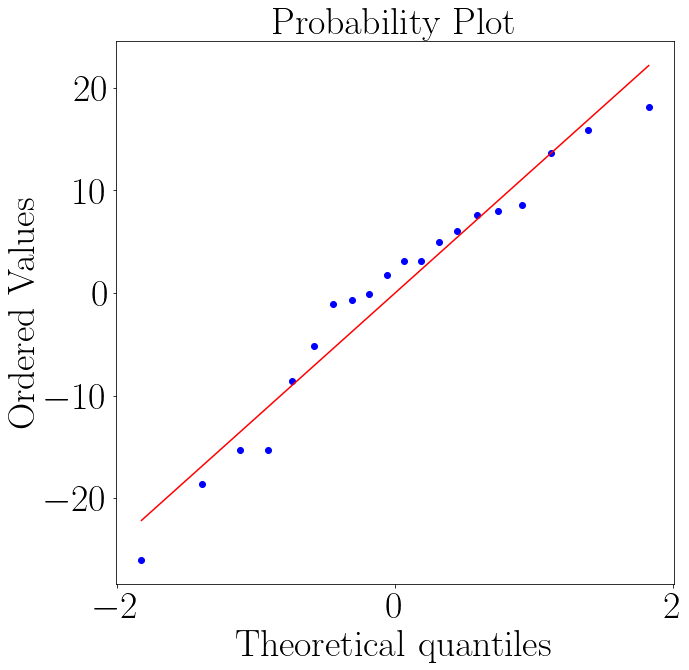
\includegraphics[width = 0.8\linewidth]{Resultados/Nasa/Figuras/png/qqplot_nasa_var.png}
        \caption{Bar plot of the average NASA-TLX score of the blind participants on each method.}
        \label{fig:qqplot_nasa_var}
    \end{minipage}
    \begin{minipage}{0.45\textwidth}
        \centering
        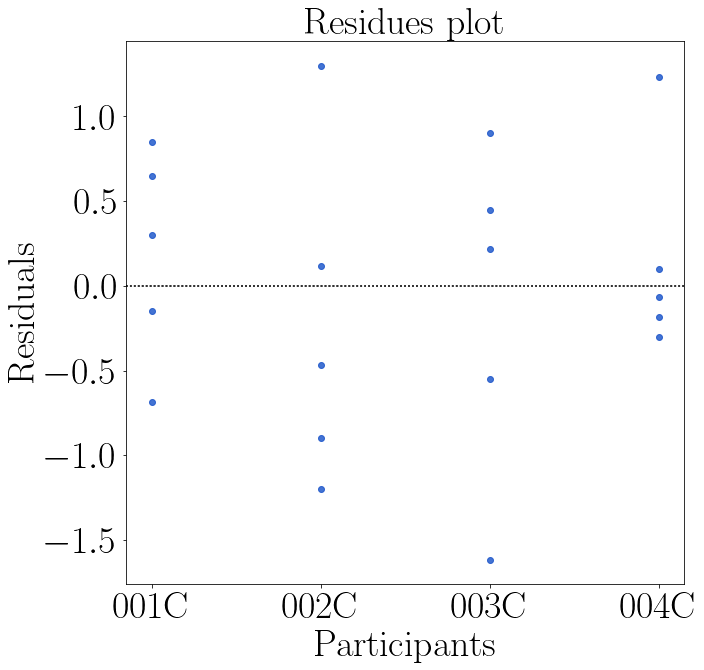
\includegraphics[width = 0.8\linewidth]{Resultados/Nasa/Figuras/png/residplot_nasa_var.png}
        \caption{Bar plot of the average NASA-TLX score of the sighted participants on each method.}
        \label{fig:residplot_nasa_var}
    \end{minipage}
\end{figure}

%The Table \ref{tab:lsdbloc_nasa_var} presents the conclusion of a pairwise Fisher LSD test of the blind NASA-TLX score between all the guidance methods. The results show that all methods have similar variations.

%
\begin{table}[!htb]
\centering
\caption{Cross validation p-value for the NASA-TLX score variation on each method for blinded users.}
\label{tab:lsdbloc_nasa_var}
\begin{tabular}{rclr}
\toprule
      \multicolumn{3}{c}{Method} &                                       Analysis \\
\midrule
              Base & $X$ & Audio &           $H_1 : \mu_{Base} \ne \mu_{Audio}**$ \\
        Base & $X$ & Haptic Belt &         $H_0 : \mu_{Base} = \mu_{Haptic Belt}$ \\
       Base & $X$ & Virtual Cane &    $H_1 : \mu_{Base} \ne \mu_{Virtual Cane}**$ \\
            Base & $X$ & Mixture &             $H_0 : \mu_{Base} = \mu_{Mixture}$ \\
       Audio & $X$ & Haptic Belt &    $H_1 : \mu_{Audio} \ne \mu_{Haptic Belt}**$ \\
      Audio & $X$ & Virtual Cane &   $H_1 : \mu_{Audio} \ne \mu_{Virtual Cane}**$ \\
           Audio & $X$ & Mixture &            $H_0 : \mu_{Audio} = \mu_{Mixture}$ \\
Haptic Belt & $X$ & Virtual Cane & $H_0 : \mu_{Haptic Belt} = \mu_{Virtual Cane}$ \\
     Haptic Belt & $X$ & Mixture &  $H_1 : \mu_{Haptic Belt} \ne \mu_{Mixture}**$ \\
    Virtual Cane & $X$ & Mixture & $H_1 : \mu_{Virtual Cane} \ne \mu_{Mixture}**$ \\
\bottomrule
\end{tabular}
\end{table}



To close up, according to the LSD test at Table \ref{tab:lsd_nasa_avg_two_way} only the "Audio" method has a NASA-TLX score that could be said to be similar to the "Base" method, which indicates that the existance of an haptic device increased the NASA-TLX score and that the round has some impact on the score, which means that there was a learning effect from the "First" to the "Return" round. Probably this effect was reflected in the other dimensions of the NASA-TLX.

The \ref{tab:blocanova_nasa_avg_two_way} concludes that the rounds and the interaction between the rounds and the methods have no influence on the variation of the NASA-TLX score.

\FloatBarrier